\subsection{Rate eligibility and read-history-aware response development}
\label{sec:he0435-response-repair}

The preceding first extraction contains a specific pixel-selection error.
For the archived native JWST/NIRCam \texttt{CAL\_VER=2.0.1} rate products,
\texttt{SATURATED} can report saturation in a later group while earlier
groups still supply a usable slope \citep{STCalChanges}.
Rejecting every such rate discards
information. An additive, release-checked adapter retains a slope only
when SCI and ERR are finite, ERR is positive and \texttt{DO\_NOT\_USE}
is absent. It checks native two-dimensional ImageModel/rate provenance
and completed ramp fitting; it does not apply this rule to raw GROUPDQ,
mosaics or unverified releases. The original fitter, SCI/ERR/DQ arrays
and frozen checkpoints are preserved.

The supplied repair package cited the correct immutable source revision
but carried a legacy-fitter digest inconsistent with that revision.
Its default guard rejected the replay before data application. A
separate integration manifest binds the actual original Git object and
the same ten JSON inputs; it changes neither the fitter nor any physical
prediction. The delivered files and failed guard remain archived.
Canonical native-coordinate replay then reproduces all sixteen original
centroids exactly in the current runtime. This is an explicit provenance
correction, not a silent relaxation of an input check.

The verified adapter restores 303 valid slope pixels. With the original
fixed library response, the G1-reference raw $q$ RMS becomes
$0.448457055$ mas and the R1-inclusive value $0.448562655$ mas.
The exposure statistic becomes $253.027695$ for 15 coordinates.
All sixteen absolute profile checks still fail, with quadratic residual
per degree of freedom $27.57$--$83.55$. Restoring information tightens
conditional centroid errors: the G1-reference formal geometry statistic
is $1033.114$ for five coordinates despite its smaller raw discrepancy.
The original $0.779400$ mas result remains the historical first extraction;
the correction is a development reanalysis of the same photons.

The package also contains completed response trials, preserved as delivered
rather than rerun here. A positive field-trained response transfers partly,
giving about $0.362$ mas raw RMS, but held field and target profiles fail.
Finer response bases, limited spatial gradients, local-quasar calibration,
dated optical color/diffusion and eight bounded pupil-phase modes also
remain inadequate. Those prior trials do not authorize a new arbitrary
PSF family or a coefficient fitted to the gravitational residual.

The delivered native detector-history calculation supplies a more specific
lead. A numerically compatible \texttt{stcal 1.18.0} ramp fit reproduces
the archived field rate and ERR within $8.97\times10^{-8}$ and
$1.65\times10^{-7}$ relative, respectively. The archived installation
version is not recorded; numerical agreement is not proof of that
installation history. The earlier incompatible replay is retained.
That completed field experiment is retained. The new target/exposure
applications below recover the additional histories on their actual domains.
On exactly 289 matched field-star pixels, a separately calibrated
first-two-read difference reduces normalized raw profile residual from
$7.6653\%$ to $5.1787\%$. Its $p=0.00984653$ still fails the declared
$0.01$ gate, formal centroid errors grow about threefold, and several
wing annuli worsen. Neither the lower quadratic statistic nor a
shorter common-time extraction is promoted to validation.

The image operator must therefore expose the consumed histories and
extended light. For a conditional BHSM sky and instrumental parameters
$\eta$, the native pixel mean has the evaluated structure
\begin{align}
 I(\theta,\lambda)&=\sum_i F_i(\lambda)
          \delta^2(\theta-q_i)+\sum_k a_k(\lambda)B_k(\theta),\nonumber\\
 f_{ep}&=\int\!\dd\lambda\,T_e(\lambda)
            \int\!\dd^2\theta\,
            P_{ep}(\theta,\lambda;\eta)I(\theta,\lambda),
 \label{eq:he0435-scene-native-operator}
\end{align}
followed by the read-accumulation and slope-estimation operator.
Here $P_{ep}$ already includes the native pixel integral. The sky
quadrature in this equation integrates over source position and does
not integrate that pixel response a second time. The frozen optical
map supplies the physical predicted point positions; during response
development the measured $q_i$ are independent nuisance coordinates.
Agreement with a lens prediction is never the calibration objective.
The shared observed-sky basis describes only the sampled neighborhoods;
these disjoint stamps do not uniquely reconstruct galaxy and lensed-host
light over the full field.

With the actual individual read times $t_{jr}$, we evaluate the
following leading time/illumination candidate:
\begin{align}
 \mathbb E[G_{pj}]&=a_{p,s(j)}+\langle t\rangle_j f_p
            +\frac{\kappa_e}{2g_p}\langle t^2\rangle_j
                    [L((gf)^2)]_p,\label{eq:he0435-read-history-candidate}\\
 \mathbb E[\widehat f_p]&=f_p+
       \frac{\kappa_e}{2g_p}\sum_j w_{pj}\langle t^2\rangle_j
                    [L((gf)^2)]_p .\nonumber
\end{align}
The symmetric neighbor-exchange graph $L$ has zero total flux, so this
candidate conserves charge at each read on its specified domain.
Pixel-specific slope weights can nevertheless yield a nonconserved sum
of the final slopes; renormalizing those slopes would hide the history
dependence. DNU and SAT exclude a group, while a jump starts a new
intercept segment. The actual group average of $t^2$, rather than the
square of the group mean time, is required. For static linear response,
the group-estimator identities $w_p^TH_p=0$ and $w_p^Tm=1$
eliminate segment intercepts $H_p a_p$ and return $f_p$;
different histories alone cannot alter a static linear profile.
The second line of Equation~\eqref{eq:he0435-read-history-candidate}
is this linear group-estimator identity. Those first direct-group applications did not reconstruct archived OLS\_C
weights or individual ZEROFRAME branches. The subsequent native applications
below retain the actual adaptive estimator and ZEROFRAME selection.
This candidate is a specified leading response hypothesis, not a
uniquely derived charge-migration law or a measured detector constant.
In this direct-group application $f_p$ is in corrected DN s$^{-1}$,
$g_p$ is the recorded gain in electrons per DN and $\kappa_e$ is in
electron$^{-1}$. The graph acts on accumulated electron charge; conserving
DN alone would not conserve charge when the gain varies. Fixed flat and
photometric maps convert the optical surface-brightness prediction to
the count units. An initial DN-conserving surrogate is retained as a
superseded development implementation, with its unit correction explicit.
The delivered gain is spatially constant at $2.05$ electrons/DN, so its
predicted means coincide with the corrected electron formulation after
rescaling the coefficient. A nonuniform-gain regression checks the
general conservation law; no electron leakage is inferred for this
particular constant-gain data set.

Shared reads also require temporal covariance. Under an independent post-correction
CDS-marginal working assumption \citep{JWSTReadnoise201}, the conditional photon
term for two two-read groups is
\begin{equation}
 C^{\rm ph}_{p,jk}=\frac{f_p}{4g_p}
       \sum_{r,s}\min(t_{jr},t_{ks}),
 \qquad C^{\rm read}_{p,jk}=
       \delta_{jk}\frac{R_{{\rm CDS},p}^2}{4}.
 \label{eq:he0435-group-noise}
\end{equation}
The common-read covariance must enter a held-group prediction, instead
of summing early and full-rate likelihoods as independent data.
Linearity derivatives, SIRS-induced spatial covariance, dark/reference
covariance and observed-selection effects remain distinct limitations.
Moreover, the stipulated mean exchange does not specify a stochastic
electron-transfer law, so it does not determine redistribution-induced
interpixel covariance. These are conditional mean applications with a
frozen working covariance, not a complete detector likelihood.

Learned optical-response uncertainty also induces correlations between
image centroids. With one declared SVD convention on a whitened,
dimensionless Jacobian, the local joint information must profile all
shared response and sky nuisance directions together. A fixed-PSF
two-by-two inverse information per image omits those correlations.
All resulting uncertainty statements remain conditional when the mean
profile is inadequate. The following new applications assess this
functional structure on consumed development observations; none opens
a reserved band, repeats the original blinded experiment, or changes
the $2\times10^{-10}$ physical guard and false admission state.

The first executed temporal application jointly fits the first eight
groups with independent pixel rates and segment intercepts, using the
ninth group only for a conditional prediction. Its working covariance
is frozen from training-only rates and includes the shared-read term.
The ninth group was already present in the delivered observations;
this is an internal temporal holdout, not a new unused-photon test.
The fit gives $\kappa_e=2.3627\times10^{-7}$ electron$^{-1}$ with local
conditional curvature error $3.3518\times10^{-8}$ electron$^{-1}$.
Training $Q$ falls from 1621.402 to 1566.524. On 257 retained held
pixels, conditional-prediction $Q$ falls from 272.942 to 260.747 and
raw residual RMS from 10.20884 to 9.67245 DN, a 5.25\% reduction.
Free pixel rates make this a temporal-curvature diagnostic rather
than optical-profile calibration. Missing calibration/spatial
covariance prevents interpreting the curvature error as a complete
detector-coefficient measurement.

An actual coupled optical test then restricts the rate map to the
fixed dated 4000 K, equal-sampling STPSF \citep{STPSFMeasuredOPD}, free centroid and flux, and
one background plane. These six optical nuisance coordinates are
jointly fitted with $\kappa_e$ through the original group operator.
The full seven-parameter local covariance retains their correlations.
Although training $Q$ improves from 11909.177 to 11569.456, the held
group worsens: $Q$ rises from 1542.413 to 1573.909 for 257 pixels and
raw residual RMS from 25.23791 to 25.58811 DN. The fitted conditional
$\kappa_e\simeq2.3665\times10^{-7}$ electron$^{-1}$ therefore does not repair
the optical mean. This controlled failure distinguishes a measurable
temporal lead from a sufficient PSF response; no such coefficient is
transferred to quasar extraction or assigned to a gravitational term.

The separate rate-image application evaluates
Equation~\eqref{eq:he0435-scene-native-operator} with a coherent sky.
Each of the four disjoint image neighborhoods has a $3\times3$ basis
of nonnegative observed-sky Gaussians of width $0.10$ arcsec and spacing
$0.18$ arcsec. Its 36 coefficients are common to all exposures, with
a declared zero-centered Gaussian penalty of scale 10 in SCI units
restricted to nonnegative coefficients. Exact archived GWCS maps
sample that sky at one quarter of a native pixel. The already
pixel-integrated response is convolved once, with zero response
outside its declared 25-pixel support and padded sky quadrature;
the likelihood uses the canonical $17\times17$ native stamps.
One detector background plane per exposure replaces independent
quadratic backgrounds around each image. Point coordinates and fluxes
remain free measurement nuisances. No physical lens prediction is
loaded by this calculation.

The response retains the delivered positive field family with 318
coordinates:
\begin{equation}
 P(u;\eta)=\frac{\operatorname{spline}(P_0)(u)
                    \exp[B(u)\eta]}{Z(\eta)}.
\end{equation}
Its original gauge removal and finite-grid normalization are retained.
Four field-star stamps supply the calibration
likelihood; the declared coefficient prior has scale $0.2$.
The objective evaluated retains the original native residuals
\begin{align}
 r_{ep}&=\frac{d_{ep}-f_{ep}(q,F,a,\eta)
                    -b_{e0}-b_{ex}x_p-b_{ey}y_p}{\mathrm{ERR}_{ep}},\nonumber\\
 Q&=\sum_{ep}r_{ep}^2+Q_{\rm field}
             +\|a/10\|^2+\|\eta/0.2\|^2 .
 \label{eq:he0435-scene-original-residual}
\end{align}
Field flux, position and affine background are profiled at each
evaluated response. Native ERR is unchanged. This sky is a finite
observed-light nuisance description; its positive patches do not
identify the separate galaxy and source-plane host components.

First, field-only calibration uncertainty is propagated at the
delivered response. If $A$ and $B$ are the whitened point/sky nuisance
and response Jacobians and $F_p$ includes the stated sky penalty,
the cut covariance is
$C_p=F_p^{-1}+S C_{\eta,\rm field}S^T$ with
$S=-F_p^{-1}A^TB$. This retains common calibration uncertainty
without allowing target pixels to update its mean. A separate
coupled Gauss--Newton application then updates point, sky and response
coordinates together, re-profiles the field nuisances, and accepts
a step only after re-evaluating the original nonlinear
Equation~\eqref{eq:he0435-scene-original-residual}.
All ranks use singular values of dimensionless columns above
$10^{-10}$ times the largest value. Null projections and the
distinction between data rank and prior-supported rank are recorded.

The continuation is now solved to conditional stationarity with all field
nuisances included jointly. Convergence requires the largest projected
half-objective gradient, in the declared dimensionless scales, to be at
most $10^{-3}$ and the last relative objective change at most $10^{-10}$.
The all-data objective is $44420.297987$, with target raw
$Q=33639.007883$ and projected gradient $4.896\times10^{-5}$.
The joint problem has rank 438/438 including the stated priors; five sky
coefficients are on their zero bound. Its full centroid covariance
retains shared sky/response and cross-exposure terms, but remains
unconstrained local curvature under an inadequate mean.

Training on E1--E3 target stamps and all four field-star stamps also
converges: objective $34631.543686$, target $Q=23295.018884$ and
projected gradient $3.535\times10^{-4}$. With trained sky and response
fixed, the independent E4 point/flux/plane application converges but
fails: $Q=11018.981762$ for 1141 nominal conditional degrees of freedom,
compared with $10906.483$ at the old one-step iterate. Between 72\% and
85\% of each image's quadratic residual is outside three pixels.
Thus the earlier failure was not resolved by optimization convergence.
Figure~\ref{fig:he0435-joint-scene-residuals} compares this persistent
spatial pattern with the full native application below, using unchanged ERR.
\begin{figure}[!htbp]
 \begin{adjustwidth}{-\extralength}{0cm}
 \centering
 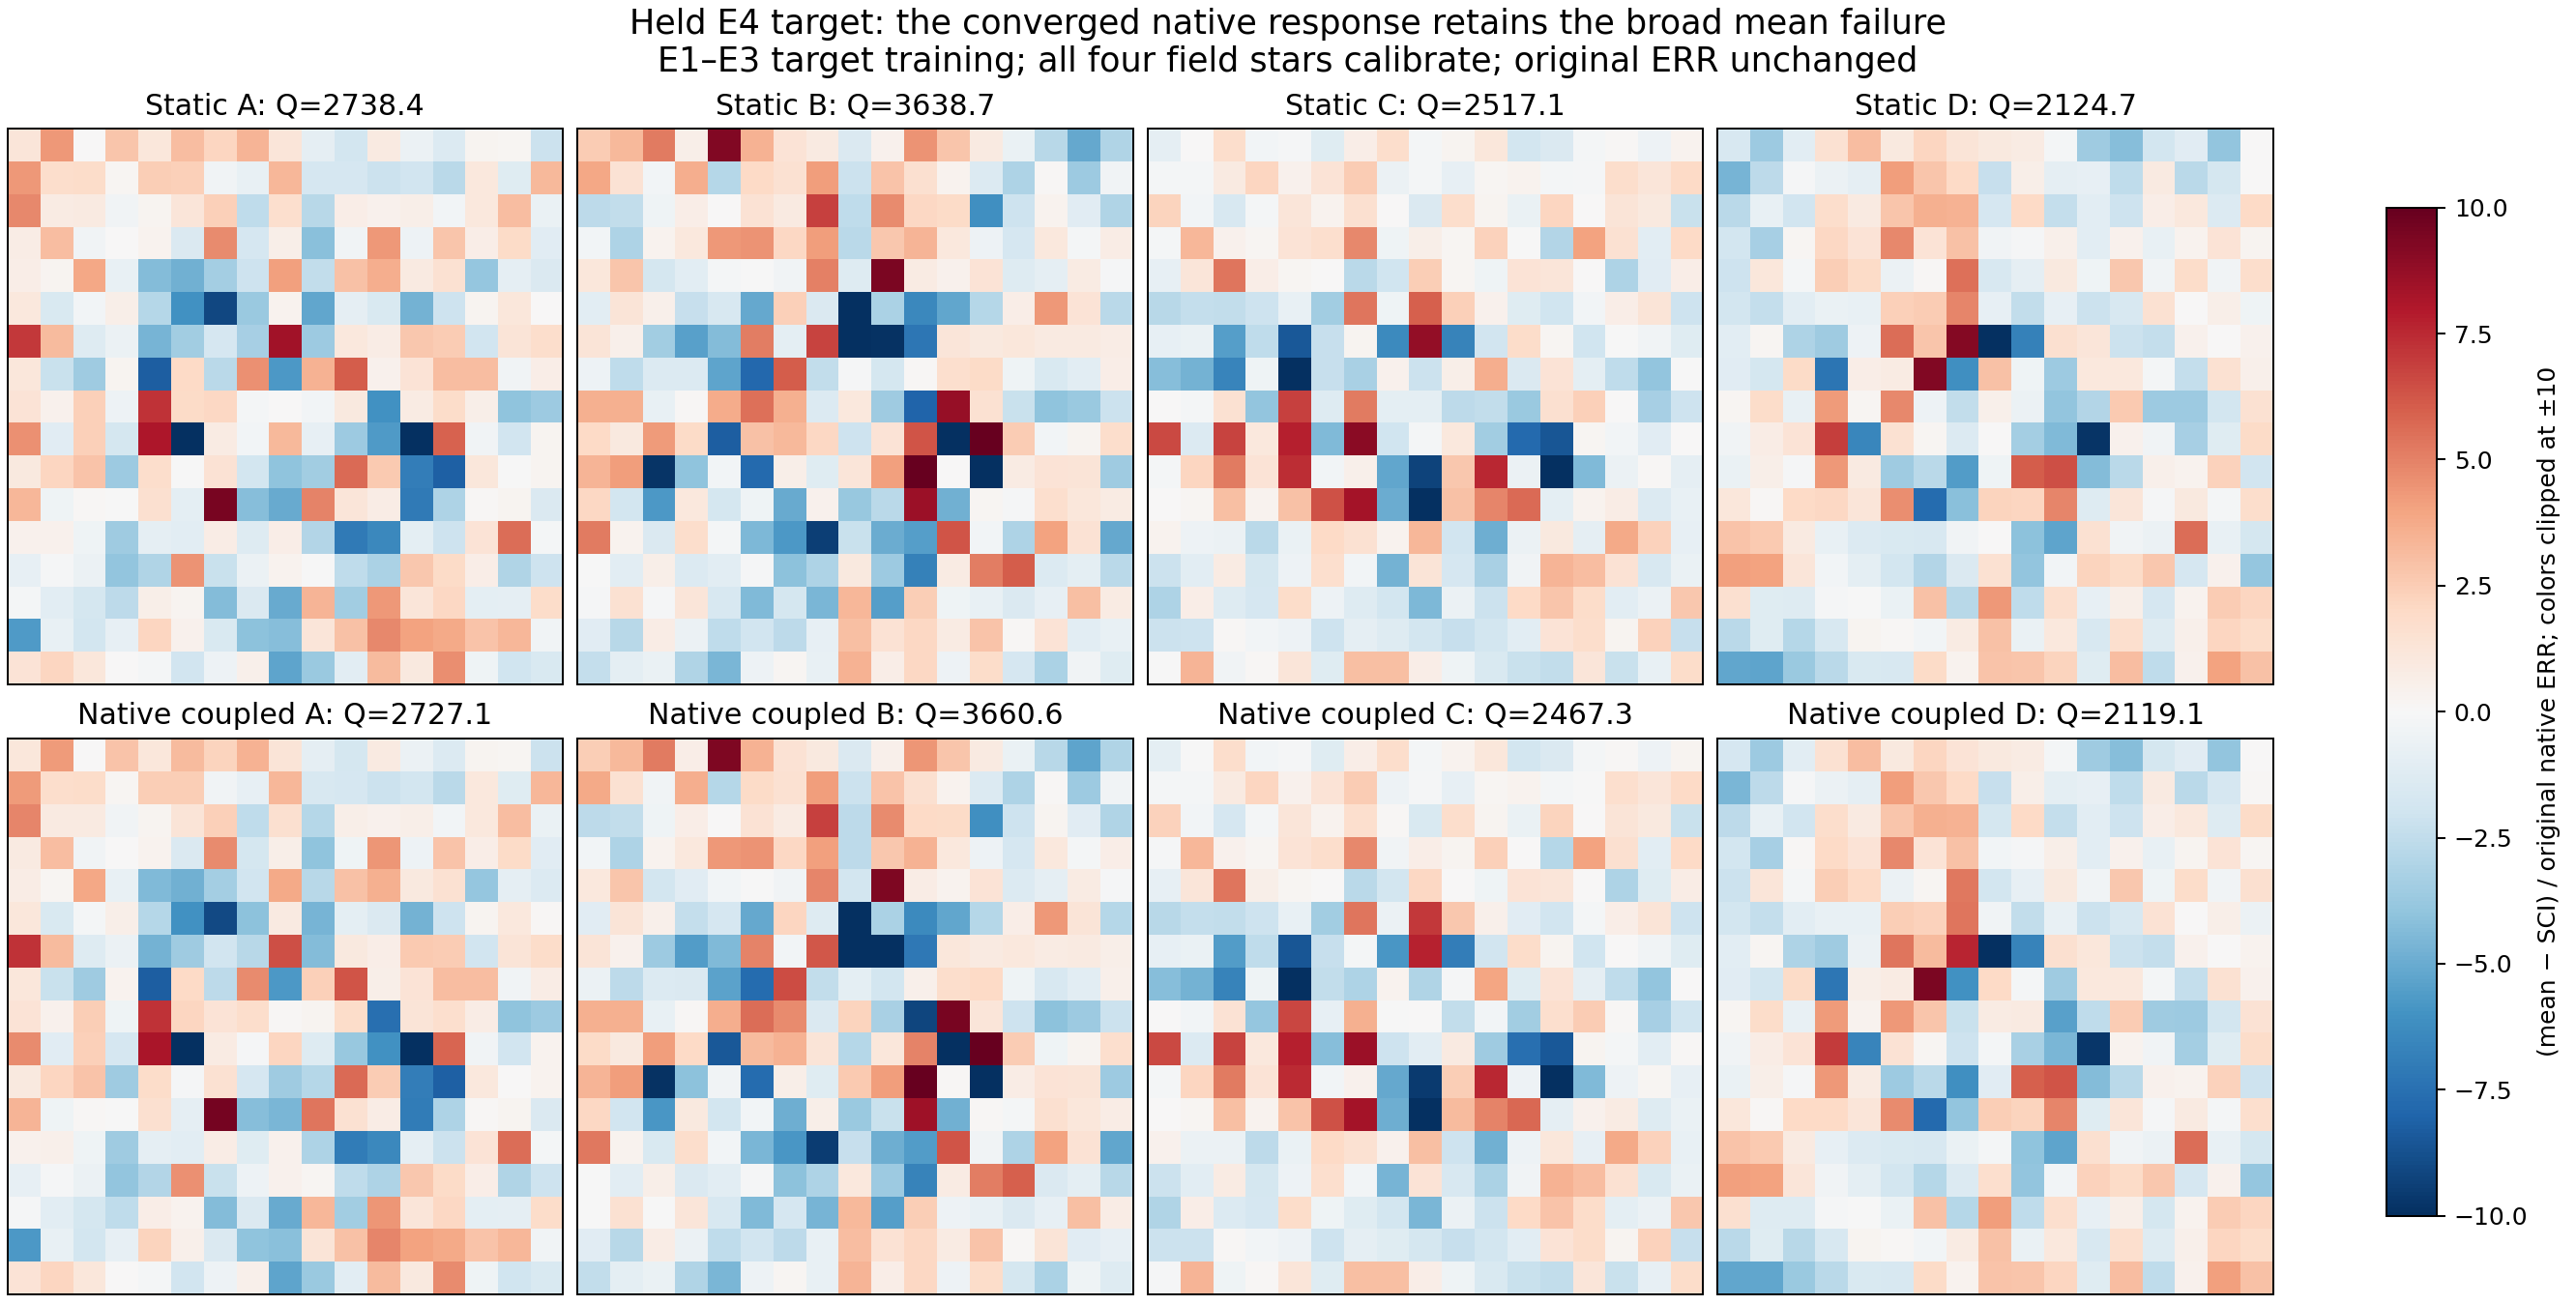
\includegraphics[width=\fulllength]{figures/he0435_converged_held_residuals_20261021.png}
 \caption{Actual held E4 native $17\times17$ target residuals at the
 converged static and calibration-ordered native sky/response fits.
 The shared response
 and coherent sky train on E1--E3 targets and all four field-star stamps;
 held point/flux/plane nuisances are fitted independently, while the
 native electronic intercept is conditioned on its observed first group. Color shows
 $(\mathrm{mean}-\mathrm{SCI})/\mathrm{ERR}$, with colors alone clipped
 at $\pm10$. Excluded pixels are masked; raw residuals and quoted
 statistics are not clipped. The native charge response lowers total
 held $Q$ by 0.41\%, leaving the broad structured
 failure. These are consumed development observations.}
 \label{fig:he0435-joint-scene-residuals}
 \end{adjustwidth}
\end{figure}

The additional native histories have now been recovered for A--D and a
field star in each of the four exposures, on matching $65\times65$
detector domains. These are nine downlinked two-frame group averages
and the first individual read as ZEROFRAME; the complete later
individual-read sequence was not downlinked.
Their known read times are retained, rather than inventing individual
observations from averages. Full-detector SIRS precedes extraction.
All twenty rate/ERR replay checks pass the original $10^{-4}/10^{-3}$
relative gates, with worst discrepancies $1.8394\times10^{-7}$ and
$1.7881\times10^{-7}$. Compact official OLS\_C exactly reproduces the
full-detector slopes. The documented runtime is
\texttt{stcal 1.18.0+winportable1}; its platform/debug portability patch
changes no slope or variance equations and establishes no archived
installation history. Reference DQ maps are interpreted through their
own DQ\_DEF, separately from the global science flags.

The native group map also matters. If $\ell_p$ is the recorded
linearity polynomial and $q_{pjr}$ a linearized read mean, the earlier
conditional per-pixel application evaluates
\begin{equation}
 \mathcal H_{pj}(q)=\ell_p\!\left[
       \frac12\sum_{r=1}^{2}\ell_p^{-1}(q_{pjr})\right]-D_{pj},
 \qquad q_{pjr}=\beta_p+\frac{\mu_p(t_{jr})}{g_p}+D_{pjr}.
 \label{eq:he0435-native-read-group-map}
\end{equation}
The electronic intercept and individual-read dark contribution enter
before inverse linearity and averaging; the native group dark is
subtracted afterwards. The inverse uses the actual anchored monotone
branch. Its read Jacobian and Hessian are evaluated explicitly.
Actual data-anchored nonlinear-averaging shifts reach 87.624 DN in a
bright core, but only 0.004558 DN per group in the 3--6-pixel wings.
This known correction cannot explain the broad wing failure alone.

The calibration source trail further specifies the operator order.
The archived-context IPC reference is a ground-derived deconvolution
kernel $G$, while the linearity reference records IPC correction
before its coefficient fit. Native science processing skips IPC.
Writing $H=G^{-1}$, the nominal physical composition is therefore
\begin{equation}
 \mathcal R_j=\ell\!\left[H\left\{
  \frac12\sum_r\ell^{-1}\!\left(\beta+
        \frac{\mu_{\rm pre}(t_{jr})}{g}+D_{{\rm pre},jr}\right)
                    \right\}\right]-D_{{\rm native},j}.
 \label{eq:he0435-calibration-ordered-ipc}
\end{equation}
The optical effective profile already includes its low-charge IPC
mean: the corresponding pre-IPC photon rate is $gG(f_{\rm eff}/g)$,
not a second convolution of the PSF. A positive Neumann inverse of
the stored $G$ has omitted kernel mass below $2.076\times10^{-15}$;
the reference's small normalization discrepancy is retained. All
twenty central $17\times17$ pre-IPC source domains are positive.
The finite field-template outer boundary requires an explicit
harmonic source continuation; its induced central low-charge change
is below $4.82\times10^{-12}$ electron s$^{-1}$ in the initial
saved-pilot application.
This nominal signal-independent reference does not fix nonlinear IPC,
full well or undocumented nonzero hot-dark calibration stages.

A matched first-two-group sky/response application converges as well,
with target $Q=7085.723398$, field $Q=1875.832461$ and projected gradient
$5.636\times10^{-6}$ under a frozen conditional photon/CDS-marginal
metric. Held E4 gives $Q=2277.353794$ and remains inadequate. Larger
sampling uncertainty in this shorter temporal projection is not a
repair, and early/full likelihoods are not summed as independent data.
The learned means are instead forwarded through
Equation~\eqref{eq:he0435-native-read-group-map} and actual native OLS\_C,
with original full-rate ERR retained as a separate comparator.

Actual raw cores plateau above the SAT calibration cutoff but below
65534 DN. Neither is a physical stored-charge measurement after
saturation. Two bounded first-order mean continuations are therefore
kept distinct. For a storage ceiling $Q_p$, define
$H_p(t)=\int_0^t\min(\lambda_p s,Q_p)\,\dd s$ and
$D_p(t)=\sum_q(\lambda_p+\lambda_q)[H_q(t)-H_p(t)]$;
then $\mu_p=\min(\lambda_p t+\kappa_e D_p,Q_p)$ explicitly loses overflow.
The electronic-ceiling alternative keeps $H_p=\lambda_p t^2/2$ and
unbounded stored charge, clipping only the readout. Both recover the
original leading mean before ceilings. Initial-intercept-translated
SAT-cutoff and 10\% larger ceilings are declared trials, not measured
full wells. Undefined positive context values receive a recorded
harmonic continuation. Group0 conditions electronic intercepts;
observed DQ/jump branches remain fixed without reconstructing deposited
cosmic-ray charge. These assumptions restrict the application.

The complete native mean is then solved jointly, retaining the same
318 response and 36 sky coordinates, all point and field nuisances,
and a nonnegative $\kappa_e$. Its derivative includes the implicit
first-group electronic intercept, translated ceiling, inverse linearity,
IPC, native linearity and the source-derived piecewise OLS\_C branches.
The positive incident-rate boundary is fixed before fitting: the inner
$33\times33$ target and $17\times17$ field domains are trusted,
with a harmonic exterior on the full 65-pixel context. An initial
compact-template-edge prescription blocked optimization and is retained
as an unsuccessful attempt, rather than a converged result.

The 439-coordinate all-data problem converges with projected gradient
$1.3215\times10^{-4}$ and $\kappa_e=1.59453\times10^{-7}$ electron$^{-1}$.
Its original target $Q$ is $33330.090404$; official float32 OLS\_C
replay gives $33330.089424$. The 424-coordinate training problem
also converges, with projected gradient $1.6477\times10^{-4}$ and
$\kappa_e=1.65400\times10^{-7}$ electron$^{-1}$. Held target E4,
with independent point/flux/plane nuisances and its electronic intercept
conditioned on observed group0 through the original boundary equation, converges
to original-ERR $Q=10974.065420$ in native replay. This 0.41\%
improvement remains grossly inadequate. Approximately 79\% of held
$Q$ lies outside three pixels; pixels without native jump flags
alone contribute $Q=9867.84$. The failure is therefore not explained
by unresolved jump deposits alone. Full train/held sky/response/charge
cross-covariance is retained as unconstrained local curvature.
These are converged conditional mean problems with the original ERR
metric, not optima of a completed illuminated-detector state likelihood.

The missing stochastic term is addressed by an explicit conditional
collection-boundary law, rather than inferred uniquely from its mean.
Set $A_{pq}=\kappa_e(\lambda_p+\lambda_q)$ on each neighboring pair and
$A_{pp}=-\sum_q A_{pq}$. Its local moment equations are
\begin{align}
 \dot\mu&=\lambda+A\mu, &
 \dot C&=AC+CA^T+\operatorname{diag}(\lambda+A\mu),\nonumber\\
 K(t,s)&=e^{A(t-s)}C(s), && t\geq s .
 \label{eq:he0435-conditional-counting-covariance}
\end{align}
These equations recover the leading mean and the $\kappa_e=0$
Poisson $\min(t,s)$ covariance. The implementation projects all
interpixel and unequal-time terms through the actual read maps on the
finite context, including source births outside selected pixels.
This is a declared local affine/linear-noise completion, with explicit
small-signal and charge-domain checks, not an exact stochastic overflow
law or a microscopic BHSM state kernel. A mean-dependent Gaussian
instrument likelihood requires $\log\det C$ and covariance derivatives;
its full score is implemented separately from frozen-$C$ continuation.

Reference noise has an actual source constraint. The observed-mask SIRS
Jacobian retains top/bottom odd/even offsets, calibrated side kernels,
rejection masks and shared cross-stamp columns. All 36 native group
corrections reproduce pre-to-post pixels bitwise. However, READNOISE0282
was estimated after reference, bias and IPC correction. Its delivered
CDS diagonal therefore does not identify independent raw ADC noise.
Adding a second reference variance to that diagonal would omit
science/reference cross terms and may double count noise. The required
relation is $C_{\rm post}=C_{ss}+JC_{rr}J^T-C_{sr}J^T-JC_{rs}$.

The reference HISTORY names calibration dark programs 1453 and 4442.
Two public full-frame NRCB3 RAPID exposures from program 1453, with two
integrations each, now supply actual matched 18-read supports spanning
all nine groups. Native bias/SIRS correction is applied without IPC
deconvolution. Integration differences and declared spatial-frequency
pooling estimate the joint science/reference covariance independently
of lens residuals. The cross-covariance identity closes within
$1.09\times10^{-10}$ DN$^2$. Post-correction nearest-neighbor covariance
of 20--41 DN$^2$ and horizontal lag-64 covariance of 5--12 DN$^2$ show
that diagonal-only noise is incomplete. Training the first epoch and
testing the last gives variance ratios 0.698--0.819; this transfer
variation remains explicit. Spatial stationarity, independent
integrations and finite calibration sampling remain conditional inputs.
No fitted variance multiplier is used to certify a failed mean.

An actual full cross-stamp/amplifier covariance application replaces
the old native read-variance component with that measured source
component; it does not add a second copy of read noise. Exact
source-derived native branch derivatives replace finite-step derivatives
that crossed adaptive estimator branches. The saved static held target
mean then has conditional $Q=3901.2783$ on 1156 pixels, with its raw
RMS unchanged at 1.525146 SCI units: it still fails. A separate actual
E4A contraction propagates the nonlocal noisy group0 intercept and
science/reference cross terms. It retains the translated-cap noise
path as a distinct unresolved boundary contribution. Neither calculation
turns changed uncertainties into evidence that the optical mean is correct.

Two explicit mean counterfactuals further test this failure. Moving the
entire fitted electronic plane into photon carriers before collection
and IPC, with the intercept re-solved from group0, changes held native
$Q$ only from $10974.065420$ to $10972.215765$ (0.017\%). A separately
frozen E4A experiment uses sixteen outside-ROI pixels and seven temporal
contrasts per pixel that remove a constant and linear rate. The independently
measured dark covariance predicts the target noise mean from these 112
controls, without fitting target residuals. Under its stated Gaussian
READ+DARK law, the predicted mean has RMS 0.010565 SCI units; raw target
RMS changes only from 1.299277 to 1.299070, and original-ERR $Q$ worsens
from 3385.7513 to 3425.0588. Including nominal Poisson control contamination
as a best linear predictor leaves the conclusion unchanged. Neither
background repartition nor this correlated-noise mean repairs the profile.

The remaining illuminated-detector relation is substantive. The measured
dark law and low-charge IPC reference do not specify signal-dependent
carrier redistribution, nonlinear IPC or stochastic overflow at a physical
well boundary. Even a conservative symmetric exchange with rate $h$ on
an edge changes no mean but adds $2h\,vv^T$ to the covariance rate,
where $v$ transfers one electron between its endpoints. Thus a mean
equation alone cannot determine that covariance. This observation proves
nonuniqueness; it is not an added physical exchange model. The translated
cutoff additionally consumes the joint raw/group0/reference-control
noise law. These inputs must be calibrated or declared explicitly before
a full state-dependent likelihood can be optimized. The conditional
moment law above, ground IPC and dark data fix specific parts, not that
complete illuminated boundary law.

These applications recover the histories, converge the declared
static, early and native conditional means, and evaluate omitted covariance
relations. They do not identify a unique post-saturation collection or
source/background photon-partition law. The original native residuals
remain the adequacy evidence before any reserved observation is opened.
The microscopic state/source and same-domain Cauchy conditions in the
Discussion are separate from these instrumental relations.
